\documentclass[11pt]{article}

\usepackage{amsmath}
\usepackage{amssymb}
\usepackage{bbm}
\usepackage{booktabs}
\usepackage{natbib}
% \usepackage{color}
\usepackage{caption}
\usepackage{float, afterpage, rotating, graphicx}% Including fig and tab
\usepackage{epstopdf}% Convert eps to pdf, graphicx needs to be loaded before
\usepackage[dvipsnames]{xcolor}
\usepackage[onehalfspacing]{setspace}
\usepackage{geometry}
    \geometry{margin=1.2in}
\usepackage{hyperref}
    \hypersetup{colorlinks=true, linkcolor=black, anchorcolor=black, citecolor=black, filecolor=black, menucolor=black, runcolor=black, urlcolor=MidnightBlue}
\newcommand\fnote[1]{\captionsetup{font=scriptsize}\caption*{\textsl{Note:} #1}}
\newcommand\fnotes[1]{\captionsetup{font=scriptsize}\caption*{\textsl{Notes:} #1}}
\newcommand{\todo}[1]{\textbf{\textcolor{red}{TODO: #1}}}


\title{Whitepaper: Lykke Crypto Index 20}
\author{
Onno Kleen\thanks{Heidelberg University, Department of Economics, \href{mailto:onno.kleen@awi.uni-heidelberg.de}{onno.kleen@awi.uni-heidelberg.de}}
\and
Christopher Zuber\thanks{Heidelberg University, Department of Economics, \href{mailto:christopher.zuber@awi.uni-heidelberg.de}{christopher.zuber@awi.uni-heidelberg.de}}
}
\begin{document}
\maketitle

\begin{abstract}
    Cryptocurrencies have gained increasing attention and momentum in prices during the last months.
    To measure cryptocurrency market movements as a whole, we propose the Lykke Crypto Index 20 (LCI20) to be a weighted average of the 20 largest cryptocurrencies' market capitalization.
    The purpose of our index is to closely follow the value of cryptocurrencies both to reflect short-term movements and long-term trends.
    We address cryptocurrency-specific challenges as there are, for example, the distinct market behavior around currency splits and suggest to track index evolution in real time.
\end{abstract}


\section{Introduction}

The increasing share of people trading cryptocurrencies and the increasing amount of cryptocurrencies itself make it desirable to have an index which is able to track long-term trend as well as short-term movements.\footnote{Code and PDF can be found at \href{https://github.com/onnokleen/crypto-index}{GitHub}.}
To fill this gap, we propose the Lykke Crypto Index 20 (LCI20) to be a weighted average of the 20 largest cryptocurrencies' market capitalization.
The index is set up in real time such that its composition can change, for example, if another currency overtakes the 20th index currency in terms of market capitalization.

We proceed as follows:
First, the notation is introduced.
Second, we introduce how the index is calculated.
Third, we present a reduced-form example of our index on daily data in a subsequent section.
Finally, pros and cons of our method are discussed.


\section{Definition}

Let $t$ denote our continuous time index starting at time $t_0$.
Moreover, $\mathcal{C}_t \in \mathbb{N}$ is the set of coins that are tradable at time $t$ across $M \in \mathbb{N}$ relevant market places for crypto-assets.
The price $p_{i,t}$ of cryptocurrency $i$ at time $t$ is calculated as the mean of the bid-ask spread's midpoints across all $M$ markets.
Quantity $q_{i,t}$ denotes the number of actively traded shares/items of asset $i$ at time $t$.
Last, we measure market capitalization $c_{i,t}$ by price times quantity $p_{i,t} \cdot q_{i,t}$.
Note that our definition of market capitalization depends on a proxy  called the ``public float''.
In stock market indices, only shares that are actively tradable are included in calculating those indices.
This is commonly done by excluding shares held by strategic long-term investors, e.g.\ founding shareholders or government.
So far, there is neither a systematic and publicly available recording of amounts held by strategic long-term investors nor is the amount of ``dead'' coins known.\footnote{The web is full of reports (e.g.\ \citeauthor{LetsTalkBitcoin}, 2017) where people lost their Bitcoins since they saved them on a hard drive which then got broken.
Due to the decentralized structure of most of the cryptocurrencies, these coins are lost or ``dead'' and cannot be sold at any point in the future.}
We therefore propose to weight the index with respect to the market capitalization based on coins traded in the last four years and suggest to reconsider weighting it with respect to shares of actively tradable assets when this information is available in the future.
Further, we define the weight of a single currency to be 20~\% at its maximum similarly to the approach in the German stock index DAX where the maximum share is 10~\% across 30 assets.
Since Bitcoin has right now the largest market capitalization, the effect of changes in Bitcoin prices to the LCI20 is softened.


\section{Calculation steps}

Our index is defined as a standardized ratio of weighted sums relative to its initial value:
\begin{equation}
  \text{LCI20}_t = 100 * \frac{\widetilde{\text{LCI20}}_t}{\widetilde{\text{LCI20}}_{t_0}}
\end{equation}

\noindent To calculate the index at time $t$, the following six steps are to be taken:
\begin{enumerate}
  \item Select the 20 largest cryptocurrencies by market capitalization $c_{i,t} = p_{i,t} \cdot q_{i,t}$.
  \item Calculate each coins market share $s_{i,t} = \frac{c_{i,t}}{\sum_{i \in C_t} c_{i,t}}$.
  \item Truncate market shares by maximum $\bar s$: $\bar s_{i,t} = \max\{ s_{i,t}, \bar s\}$.
  \item Rescale them, so weights sum up to one: $w_{i,t} = \frac{\bar s_{i,t}}{\sum_{i \in \mathcal{C}_t} \bar s_{i,t}}$.
  \item Calculate the weighted average $$\widetilde{\text{LCI20}}_t = \sum_{i \in \mathcal{C}_{t}} w_{i,t} c_{i,t}$$
  \item The initial value of the weighted sum is given by $$\widetilde{\text{LCI20}}_{t_0} = \sum_{i \in \mathcal{C}_{t}} w_{i,t_0} c_{i,t_0}$$
  \item Calculate the index normalized to 100 in $t_0$ over time $t$. % $Divisor = \widetilde{\text{LCI20}}_{t_0}$
\end{enumerate}


\section{Data exercise}

Cryptocurrencies have experienced an upswing in the last months.
For illustration of the strengths of our proposed LCI20, we employ our definition on real-world data.
Even though our index is defined in real-time prices, we use daily data due to limited availability of high-frequency time series.
The data contains daily closing prices and market capitalization, both downloaded from \cite{CoinCap} via their Rest API.
It includes at least 21 up to 32 different cryptocurrencies per day between November 1, 2016 to September 19, 2017 from which we choose the 20 currencies with the largest market capitalization at that specific date according to the description above.\footnote{We exclude seven days on which there is no price for Bitcoin or Ethereum.}
In our exercise, the shares are truncated at a maximum $\bar s = 0.2$.
Base date $t_0$ is November 1, 2016.

Figure~\ref{f:lci20} shows the evolution of our proposed index and Bitcoin's market capitalization share over the last 11 months at a daily data basis.
Our index increases from November 2016 to mid of September 2017 by 313~\%.
Several new currencies have been introduced/split and gained sizable market capitalization shares.
Bitcoin Cash split from Bitcoin in August 2017 and has a current market capitalization share of 6.5~\%.
Therefore, Bitcoin's market capitalization share decreased from higher than 90~\% in November 2016 to below 50~\% now.
Figure~\ref{f:curshares} depicts the market capitalization shares for the five most important currencies (in terms of market shares today).

\begin{figure}[p]%
    \centering%
    \caption{Evolution of LCI20}\label{f:lci20}%
    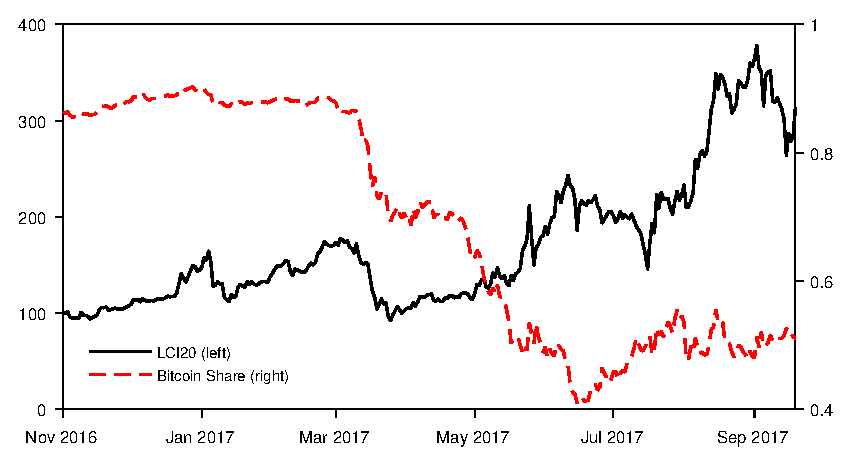
\includegraphics[width=.8\textwidth]{figs/lci20.eps}%
    \smallskip\newline% Separate caption and notes
    \fnotes{The figure shows the index value of LCI20 on the left scale. It is normalized to 100 in November 1, 2016. The market capitalization share of Bitcoin, sometimes called ``Dominance Index'', is on the right scale.}
\end{figure}

\begin{figure}[p]%
    \centering%
    \caption{Currency shares along 2017}\label{f:curshares}%
    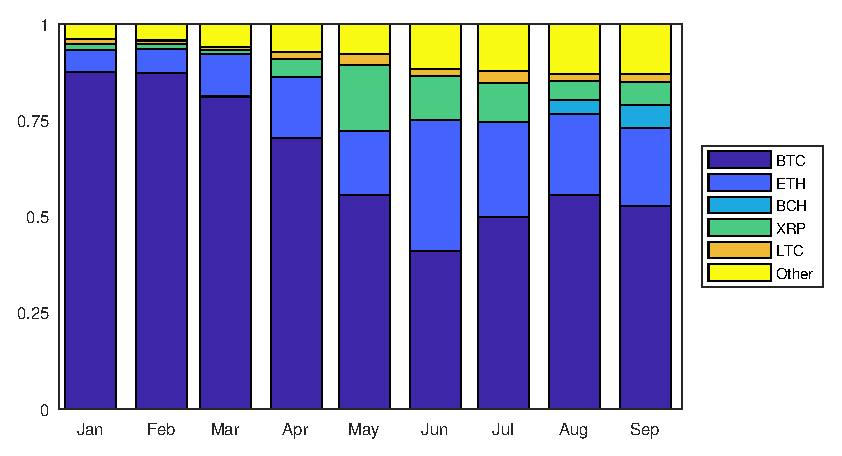
\includegraphics[width=.8\textwidth]{figs/currency_shares.eps}%
    \smallskip\newline% Separate caption and notes
    \fnotes{Individual market capitalization as share of the total market capitalization measured on the 15th of the respective month.}
\end{figure}


\section{Discussion}

 Due to the predominance of Bitcoin, one concern could be that the index is redundant if one follows just the Bitcoin price instead of LCI20.
 Figure~\ref{f:lci20vsBTC} shows that both the index and the price of Bitcoins evolve similarly but diverge over time since Bitcoin's share of market capitalization falls.

 \begin{figure}[ht]%
     \centering%
     \caption{LCI20 vs.\ Bitcoin price}\label{f:lci20vsBTC}%
     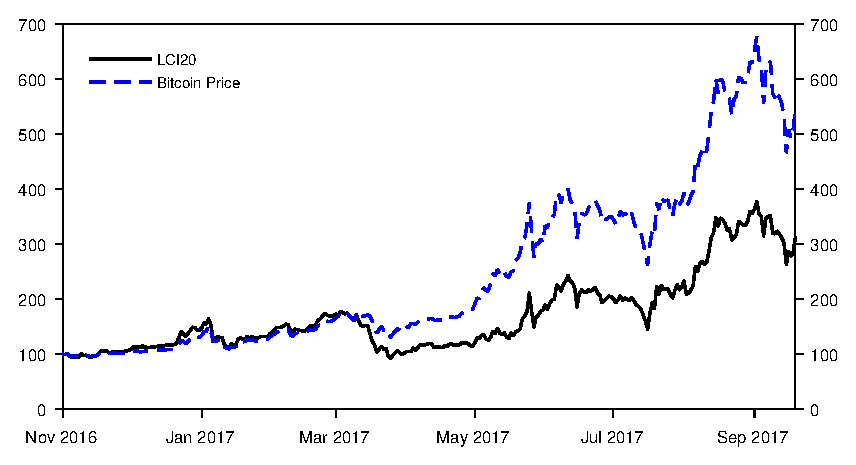
\includegraphics[width=.8\textwidth]{figs/lci20_vs_btc.eps}%
     \smallskip\newline% Separate caption and notes
     \fnotes{LCI20 and Bitcoin price is normalized to 100 in Nov 1, 2016.}
 \end{figure}

In comparison to CRIX by \cite{Trimborn2016}, we choose the LCI20 to include 20 cryptocurrencies at each point in time.
They are sorted by market capitalization from high to low and the index will consist always of the first twenty.
This has the advantage that the index represents always the 20th most ``important'' crypto-assets.
On September 22, these set of currencies had a share of 92 \% of the total market capitalization and a 24 hour trading volume of 94 \% of the total trading volume in our data set.
If we add another 30 currencies, the 24 hour trading volume increases only by 2 percentage points and the index value does only change marginally.
We therefore prefer a smaller but better traceable index consisting of 20 cryptocurrencies.

We suspect that with intra-day data, the volatility of the index increases in times shortly before and after a split.
For the daily data we use, this is not an issue as it can be seen in Figure~\ref{f:split} for the example of the split of Bitcoin Cash.
The index dropped on August 2, 2017, the day after the hard fork of Bitcoin Cash by $-10$~\% which is due to the price drop of Bitcoin ($-5$ \%) and the lower price of Bitcoin Cash (roughly 1/6 of Bitcoin).
At this point, investors which held Bitcoin, get the same amount of Bitcoin Cash.
However, both currencies share the same transaction history.
If one incautiously pushes now a transaction containing only old coins to the wrong transaction chain, one will loose the pushed value in both currencies.
Therefore, private investors are usually advised not to trade their old coins or newly gained currency in the days after a split but to wait until it is settled if the new currency becomes accepted.

\begin{figure}[ht]%
    \centering%
    \caption{LCI20 at Bitcoin Cash split}\label{f:split}%
    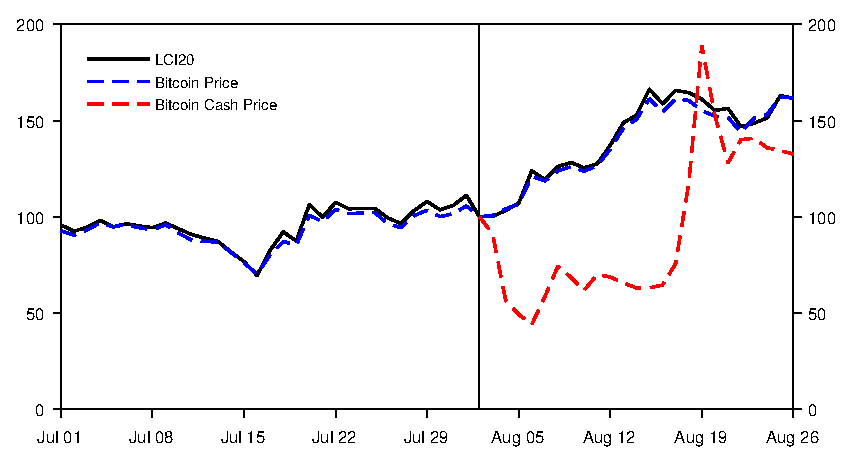
\includegraphics[width=.8\textwidth]{figs/lci20_bch_split.eps}%
    \smallskip\newline% Separate caption and notes
    \fnotes{LCI20 and prices are normalized to 100 in Aug 2, 2017.}
\end{figure}

Immaturity of markets may lead right now to frequent changes of assets included in the lower ranks of our index.
However, we want our definition of the LCI20 to be ``future-proof'' and expect volatility among ranking of crypto-assets in terms of market capitalization to decrease in the upcoming two years.






% \section{Conclusion}\label{sec:conclusion }
%For anticipated splits/forks we propose an adaptive smoothing technique for addressing ``insane'' price movements in direct aftermath.
%We propose to use one-hour averaged prices for currencies that are anticipated to split when calculating LCI20 beginning one day in advance and ending one day after split

%
%\subsection{Questions to address}
%\begin{itemize}
%
%  \item Done: ``Dead coins'' a problem?
%  \item Done: How to get market capitalization of public float? Wikipedia:  In general, the large holdings of founding shareholders, corporate cross-holdings, and government holdings in partially privatized companies are excluded when calculating the size of a public float. https://www.coindesk.com/rethinking-bitcoin-market-cap/: In 2014, NVIDIA engineer John Ratcliff theorized that approximately 30\% of the current bitcoin supply is made up of ``zombie'' bitcoins that have been inactive for more than a year This number includes bitcoins connected to inaccessible wallets, government-seized bitcoins, ``burned'' bitcoins and bitcoins abandoned during the early days of bitcoins, including Nakamoto's mythical stash of over a million bitcoins.
%\end{itemize}


%\begin{table*}
%\caption{Proposal vs.\ example}
%\centering
%\resizebox{\textwidth}{!}{
%\begin{tabular}{lll}
%  Issue & Our proposal & Example \\
%  \midrule
%  Frequency & Real-time & Daily \\
%  Split-smoothing & Not necessary due to real-time weighting & Not necessary due to daily data\\
%  Public float & Only use coins that have been traded the last 4 years & Not implemented \\
%  ``Zombie coins'' & Only use coins that have been traded the last 4 years & Only use 0.30\% of coins\\
%\bottomrule
%\end{tabular}
%}
%\fnotes{In this table differences in implementation of our example and our actual proposal are reported. Problems addressed in our proposal are reported in the first column, our solution to these in are summarized in the second column and last, we report our reduced-form example's compromise.}
%\end{table*}
%









\bibliographystyle{ecca}
\bibliography{crypto-index}

\end{document}
